% !TEX encoding = UTF-8
% !TEX TS-program = pdflatex
% !TEX root = ../tesi.tex

%**************************************************************
\chapter{I paradigmi imperativo e dichiarativo a confronto}
\label{cap:confronto-paradigmi}
%**************************************************************

\intro{
    In questo capitolo vengono illustrate le differenze principali nel creare un applicazione dotata di interfaccia utente con due paradigmi differenti: imperativo e dichiarativo.
    Mentre il secondo è quello usato da \emph{Flutter}, il primo è quello usato da molti altri \gls{frameworkg} e/o \gls{sdk} (per esempio su Android, nella libreria Swing di Java, nel \gls{frameworkg} \emph{Qt} per C++).
    Dato che durante il corso di Programmazione ad oggetti di questo Corso di Laurea è stato appreso il funzionamento di \emph{Qt}, è stato deciso di utilizzarlo come strumento di paragone.
}\\

%**************************************************************
\section{Introduzione all'esempio per il confronto}
\label{sec:introduzione-esempio-confronto-paradigmi}

Per presentare le principali differenze che sono presenti fra la creazione di un'interfaccia utente e la modifica dei dati visualizzati verrà utilizzato un esempio comune.\\
Viene creata una semplicissima applicazione in cui è presente un solo pulsante la cui etichetta è "Generato: $r$", dove $r \in [0, 9]$ è un numero intero randomico.\\
Alla pressione del pulsante, un nuovo numero casuale viene generato e l'etichetta del pulsante viene aggiornata.

%**************************************************************
\section{Il paradigma imperativo: il framework Qt in C++}
\label{sec:paradigma-imperativo-qt-cpp}

\emph{Qt} è uno dei \gls{frameworkg} più conosciuti per l'implementazione di applicazioni con interfacce grafiche usando il linguaggio C++.\\
Come in \emph{Flutter}, anche in \emph{Qt} le componenti grafiche si chiamano widget, e rappresentano le componenti native disponibili nel sistema in cui viene sviluppata l'applicazione (pulsanti, menu, caselle di testo, ecc.).\\
Esiste in \emph{Qt} un altro modo di rappresentare un'interfaccia grafica, chiamata \emph{QML}, ma non è scopo di questo capitolo e di questo documento introdurla.\\
\textbf{N.B.} L'implementazione dell'esempio non viene fatta seguendo le \gls{bestpracticeg} di \emph{Qt} e C++, è semplicemente il minimo essenziale per avere un applicazione funzionante col minor codice sorgente possibile.

\subsection{Creazione dell'interfaccia grafica}
\label{subsec:creazione-ui-qt}

Per implementare l'esempio indicato in "\hyperref[sec:introduzione-esempio-confronto-paradigmi]{Introduzione all'esempio per il confronto}", sono necessari pochi widget: una finestra e un pulsante, rispettivamente un \emph{QWidget} e un \emph{QPushButton}.
\begin{lstlisting}
#include <cstdlib>
#include <string>
#include <QWidget>
#include <QPushButton>
#include <QApplication>
#include <QString>

using std::to_string;

// Widget che definisce i dettagli della schermata
// e come comportarsi.
class ExampleApp : public QWidget {
  Q_OBJECT
  public:
    // Costruttore
    explicit ExampleApp(QWidget* parent = 0): QWidget(parent) {    
      // Impostazione di una dimensione fissa
      // per la finestra.
      setFixedSize(150, 100);
        
      // Prima generazione del numero casuale.
      r = rand() % 10;
        
      // Creazione del pulsante e impostazioni
      // per il suo funzionamento.
      button = new QPushButton(QString::fromStdString("Generato: " + to_string(r)), this);
      button->setCheckable(true);
      button->show();
        
      // Collegamento alla gestione degli eventi:
      // il SIGNAL descrive l'evento, la pressione del pulsante e
      // lo SLOT descrive cosa fare alla pressione del pulsante.
      connect(button, SIGNAL(clicked(bool)), this, SLOT(buttonClicked(bool)));
    };

    // Distruttore
    virtual ~ExampleApp() {};
    
  private slots:
    // Gestore dell'evento "Pressione del pulsante"
    void buttonClicked(bool _) {
      r = rand() % 10;
      button->setText(QString::fromStdString("Generato: " + to_string(r)));
    };
  private:
    int r;
    QPushButton* button;
};
\end{lstlisting}
Riassumendo, nella classe \texttt{ExampleApp}, che estende \texttt{QWidget}, viene:
\begin{itemize}
    \item definita la schermata stessa, impostando delle dimensioni fisse;
    \item generato il valore di $r$ iniziale e assegnato all'etichetta del pulsante nella sua creazione;
    \item impostato che il pulsante è cliccabile e reso visibile;
    \item connesso esplicitamente l'evento\footnote{Ciò che nella programmazione ad eventi è chiamato \emph{evento}, in \emph{Qt} è chiamato \emph{signal}.} \emph{clicked} con il \emph{callback} definito a livello di classe \texttt{buttonClicked}.
\end{itemize}
Quello che succede alla pressione del pulsante è la generazione di un evento \emph{clicked} e l'esecuzione del \emph{callback} \texttt{buttonClicked} che, avendo il riferimento al pulsante, ne imposta esplicitamente la nuova etichetta.

\subsection{Creazione del punto di ingresso}
\label{subsec:creazione-main-qt}

Definita \texttt{ExampleApp}, va definita la funzione \texttt{main}, il punto d'ingresso del programma:
\begin{lstlisting}
#include "ExampleApp.h"

// Main in cui viene avviato il programma e la schermata.
int main(int argc, char** argv) {
  // Inizializzazione schermata Qt.
  QApplication app(argc, argv);

  // Creazione della finestra.
  ExampleApp* exampleApp = new ExampleApp();
  exampleApp->show();

  return app.exec();
}
\end{lstlisting}
Quello che avviene in questo \texttt{main} è molto semplice: viene istanziato un oggetto di \texttt{QApplication}, che è un manager dell'interfaccia grafica in \emph{Qt}, e viene dichiarata un'istanza di \texttt{ExampleApp}, successivamente visualizzata tramite il metodo \texttt{show}.\\
L'applicazione realizzata è la seguente:
\begin{figure}[!h] 
  \centering 
  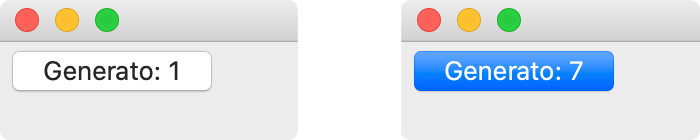
\includegraphics[width=1.0\columnwidth]{capitolo-5/qt} 
  \caption{Esempio in \emph{Qt} - Applicazione prima (sinistra) e dopo (destra) la pressione del pulsante}
\end{figure}

\subsection{Osservazioni sul procedimento}
\label{subsec:osservazioni-procedimento-qt}

Quello che si vuole evidenziare utilizzando \emph{Qt} come esempio non sono tanto le classi da usare o le necessità del linguaggio su cui si basa il \gls{frameworkg}, bensì come un'operazione di cambio dello stato dell'applicazione venga eseguita ed il ragionamento dietro ad essa.\\
Con questo tipo di \textbf{approccio imperativo}, lo sviluppatore non solo deve occuparsi dello stato dell'applicazione, ma anche dell'interfaccia grafica. Infatti nelle righe 42-43 di \texttt{ExampleApp}, una volta aggiornato $r$, lo stato, si è dovuto aggiornare il contenuto visualizzato dal pulsante tramite il metodo \texttt{setText} di \texttt{QPushButton}.

%**************************************************************
\section{Il paradigma dichiarativo: Flutter}
\label{sec:paradigma-dichiarativo-flutter}

\textbf{N.B.} L'implementazione dell'esempio è ridotta al minimo indispensabile e come si potrà vedere dalle immagini l'applicazione sarà composta da un pulsante dell'intera grandezza della schermata.

\subsection{Creazione dell'interfaccia grafica}
\label{subsec:creazione-ui-qt}

Per implementare l'esempio indicato in "\hyperref[sec:introduzione-esempio-confronto-paradigmi]{Introduzione all'esempio per il confronto}", sono necessari un po' più widget, in quanto Flutter li usa in maniera intensa, ma il codice è decisamente meno verboso.
\begin{lstlisting}
// Widget che definisce la schermata.
// Essendo uno StatefulWidget non definisce il metodo build,
// in quanto compito del possessore dello stato, ossia
// la classe _ExampleAppState.
class ExampleApp extends StatefulWidget {
  State<ExampleApp> createState() => _ExampleAppState();
}

// Stato collegato al widget ExampleApp.
class _ExampleAppState extends State<ExampleApp> {
  // Nessun widget viene dichiarato in anticipo.
  // Solo le variabili che sono parte dello stato
  // vanno dichiarate.
  final random = new Random();
  int r;
  
  // Questo metodo indica cosa va fatto ogni volta
  // che lo stato di ExampleApp viene creato da zero.
  @override
  void initState() {
    super.initState();
    r = random.nextInt(10);
  }

  // Callback che viene passata ad onPressed.
  // Corrisponde allo slot privato di ExampleApp 
  // in Qt chiamato buttonClicked.
  void _buttonClicked() {
    setState(() => r = random.nextInt(10));
  }

  // Questo metodo indica che cosa mostrare a schermo.
  // Notare come i concetti di Element e RenderObject
  // non sono presenti, in quanto sono onere di Flutter.
  @override
  Widget build(BuildContext context) {
    // MaterialApp, paragonabile a QApplication.
    return MaterialApp(
      // RaisedButton, paragonabile a QPushButton.
      home: RaisedButton(
        // In Flutter il campo dati child di un widget ha sempre 
        // tipo Widget. Quindi un pulsante non contiene solo 
        // testo, ma anche qualsiasi altra cosa (in questo
        // caso, semplice testo).
        child: Text("Generato: $r"),
        // Definizione del callback da invocare
        // alla pressione del pulsante.
        onPressed: _buttonClicked,
      ),
    );
  }
}
\end{lstlisting}
Riassumendo, nella classe \texttt{ExampleApp}, che estende \texttt{StatefulWidget}, viene:
\begin{itemize}
    \item definito il widget e siccome ha uno stato, viene creato lo stato correlato;
    \item dato che lo stato del widget interessa solo a \texttt{ExampleApp}, viene dichiarato privato (al di fuori del file non è visibile);
    \item generato il valore di $r$ iniziale in \texttt{initState};
    \item impostato nel metodo \texttt{build} che cosa viene visualizzato quando il widget viene costruito (definito $state$, \texttt{build} definisce $f(state)$);
    \item dichiarato che cosa deve avvenire all'evento di pressione del pulsante.
\end{itemize}
Quello che succede alla pressione del pulsante è la generazione di un evento \emph{onPressed} che richiama il \emph{callback} (metodo \texttt{\_buttonClicked}). All'interno del \emph{callback} ci si è occupati solo di aggiornare $r$ e di indicare che il widget va ricostruito con \texttt{setState}.

\subsection{Creazione del punto di ingresso}
\label{subsec:creazione-main-qt}

Oltre alla definizione di \texttt{ExampleApp}, va definita la funzione \texttt{main}, il punto d'ingresso del programma:
\begin{lstlisting}
import 'package:flutter/material.dart';
import 'dart:math';

void main() => runApp(ExampleApp());
\end{lstlisting}
Quello che avviene in questo \texttt{main} è inserire come widget radice nel \emph{Widget tree} un'istanza di \texttt{ExampleApp}. Visto che il \texttt{main} dispone di una sola istruzione è stato possibile usare la \emph{arrow notation}.\\
L'applicazione realizzata è la seguente:
\begin{figure}[!h] 
  \centering 
  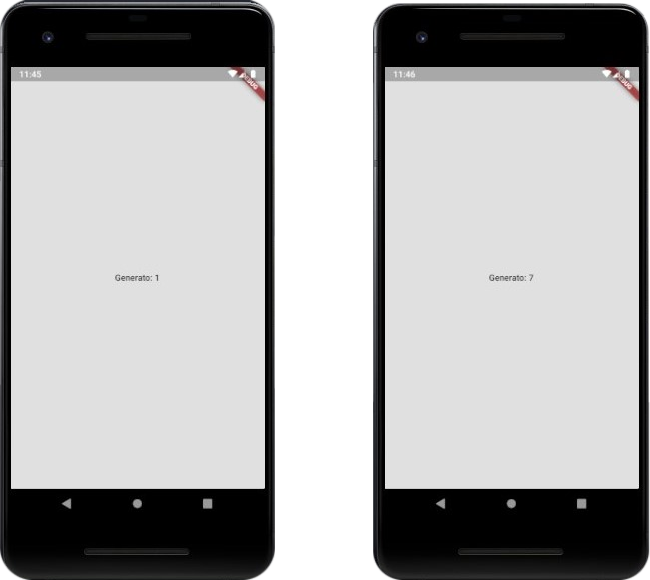
\includegraphics[width=1.0\columnwidth]{capitolo-5/flutter} 
  \caption{Esempio in Flutter - Applicazione prima (sinistra) e dopo (destra) la pressione del pulsante}
\end{figure}

\subsection{Osservazioni sul procedimento}
\label{subsec:osservazioni-procedimento-qt}

Quello che si può notare subito è la minor verbosità, sotto certi aspetti (per esempio non è necessario dichiarare che il widget va mostrato a schermo, non bisogna connettere eventi e \emph{callback} in separata sede).\\
Ma ciò che veramente conta è la separazione dei concetti.
La costruzione dell'interfaccia, basata sullo stato, è svolta solamente nel metodo \emph{build}. L'aggiornamento dello stato, svolto da \texttt{\_buttonClicked} a riga 29 di \texttt{ExampleApp}, è una pura operazione di aggiornamento stato.
Anche volendo creare un'istanza di \texttt{RaisedButton} all'esterno del metodo \texttt{build} (tecnicamente possibile) e accedendovi da dentro \texttt{\_buttonClicked}, non si sarebbe in grado di far alcuna modifica perché \texttt{RaisedButton} è un widget, e i widget sono per definizioni immutabili.
Solo richiamando \texttt{setState} è possibile informare il corrispondente \texttt{Element} che il \texttt{RenderObject} del widget va aggiornato, causando l'aggiornamento della schermata.
